%%%%%%%%%%%%%%%%%%%%%%%%%%%%%%%%%%%%%%%%%
% Journal Article
% LaTeX Template
% Version 1.3 (9/9/13)
%
% This template has been downloaded from:
% http://www.LaTeXTemplates.com
%
% Original author:
% Frits Wenneker (http://www.howtotex.com)
%
% License:
% CC BY-NC-SA 3.0 (http://creativecommons.org/licenses/by-nc-sa/3.0/)
%
%%%%%%%%%%%%%%%%%%%%%%%%%%%%%%%%%%%%%%%%%

%----------------------------------------------------------------------------------------
%	PACKAGES AND OTHER DOCUMENT CONFIGURATIONS
%----------------------------------------------------------------------------------------

\documentclass[twoside]{article}

\usepackage{lipsum} % Package to generate dummy text throughout this template
%\usepackage[caption=false]{subfig}
%\captionsetup[subfigure]{labelformat=brace}
\usepackage{graphicx, bm} % Required to insert images
\usepackage{capt-of}%%To get the caption
\usepackage{listings} % Required for insertion of code
\usepackage[usenames,dvipsnames]{color} % Required for custom colors
\usepackage[sc]{mathpazo} % Use the Palatino font
\usepackage[T1]{fontenc} % Use 8-bit encoding that has 256 glyphs
\linespread{1.05} % Line spacing - Palatino needs more space between lines
\usepackage{microtype} % Slightly tweak font spacing for aesthetics

\usepackage{amsmath}
\usepackage{amssymb}

\usepackage[hmarginratio=1:1,top=32mm,columnsep=20pt]{geometry} % Document margins
\usepackage{multicol} % Used for the two-column layout of the document
\usepackage[hang, small,labelfont=bf,up,textfont=it,up]{caption} % Custom captions under/above floats in tables or figures
\usepackage{booktabs} % Horizontal rules in tables
\usepackage{float} % Required for tables and figures in the multi-column environment - they need to be placed in specific locations with the [H] (e.g. \begin{table}[H])
\usepackage{hyperref} % For hyperlinks in the PDF

\usepackage{lettrine} % The lettrine is the first enlarged letter at the beginning of the text
\usepackage{paralist} % Used for the compactitem environment which makes bullet points with less space between them
\usepackage{titlesec}
\usepackage{cancel}

\usepackage{abstract} % Allows abstract customization
\renewcommand{\abstractnamefont}{\normalfont\bfseries} % Set the "Abstract" text to bold
\renewcommand{\abstracttextfont}{\normalfont\small\itshape} % Set the abstract itself to small italic text


\usepackage{fancyhdr} % Headers and footers
\pagestyle{fancy} % All pages have headers and footers
\fancyhead{} % Blank out the default header
\fancyfoot{} % Blank out the default footer
\fancyhead[C]{STAT-221: PSET 4 $\bullet$ November 2014} % Custom header text
\fancyfoot[RO,LE]{\thepage} % Custom footer text

%----------------------------------------------------------------------------------------
%	CODE INCLUSION CONFIGURATION
%----------------------------------------------------------------------------------------

\definecolor{MyDarkGreen}{rgb}{0.0,0.4,0.0} % This is the color used for comments
\lstloadlanguages{R} % Load Perl syntax for listings, for a list of other languages supported see: ftp://ftp.tex.ac.uk/tex-archive/macros/latex/contrib/listings/listings.pdf
\lstset{language=R, % Use Perl in this example
        frame=single, % Single frame around code
        basicstyle=\scriptsize\ttfamily, % Use small true type font
        keywordstyle=[1]\color{Blue}\bf, % Perl functions bold and blue
        keywordstyle=[2]\color{Purple}, % Perl function arguments purple
        keywordstyle=[3]\color{Blue}\underbar, % Custom functions underlined and blue
        identifierstyle=, % Nothing special about identifiers                                         
        commentstyle=\usefont{T1}{pcr}{m}{sl}\color{MyDarkGreen}\scriptsize, % Comments small dark green courier font
        stringstyle=\color{Purple}, % Strings are purple
        showstringspaces=false, % Don't put marks in string spaces
        tabsize=2, % 5 spaces per tab
        %
        % Put standard Perl functions not included in the default language here
        morekeywords={rand},
        %
        % Put Perl function parameters here
        morekeywords=[2]{on, off, interp},
        %
        % Put user defined functions here
        morekeywords=[3]{test},
       	%
        morecomment=[l][\color{Blue}]{...}, % Line continuation (...) like blue comment
        numbers=left, % Line numbers on left
        firstnumber=1, % Line numbers start with line 1
        numberstyle=\tiny\color{Blue}, % Line numbers are blue and small
        stepnumber=5 % Line numbers go in steps of 5
}

% Creates a new command to include a perl script, the first parameter is the filename of the script (without .pl), the second parameter is the caption
\newcommand{\Rscript}[2]{
\begin{itemize}
\item[]\lstinputlisting[caption=#2,label=#1]{#1.R}
\end{itemize}
}

%----------------------------------------------------------------------------------------
%	TITLE SECTION
%----------------------------------------------------------------------------------------

\title{\vspace{-15mm}\fontsize{24pt}{10pt}\selectfont\textbf{STAT-221: Pset 4}} % Article title

\author{
\large
\textsc{Kevin Kuate Fodouop}\\ % Your name
\normalsize Harvard University \\ % Your institution
%\normalsize \href{mailto:john@smith.com}{john@smith.com} % Your email address
\vspace{-5mm}
}
\date{}

%----------------------------------------------------------------------------------------

\begin{document}

\maketitle % Insert title

\thispagestyle{fancy} % All pages have headers and footers

%----------------------------------------------------------------------------------------
%	ABSTRACT
%----------------------------------------------------------------------------------------

\begin{abstract}
In this homework we use Markov Chain Monte Carlo (MCMC) methods to lead inference on the unknown number of experiments $N$ from binomial observations. Different potential priors are examined theoretically, and MCMC analysis is performed to reproduce Raftery's results (1988), in terms of posterior distribution for N, pointwise and interval estimation.

\end{abstract}

%----------------------------------------------------------------------------------------
%	ARTICLE CONTENTS
%----------------------------------------------------------------------------------------

%\begin{multicols}{2} % Two-column layout throughout the main article text

We are given n observations $Y_1, Y_2, ..., Y_n$ drawn from a distribution
\begin{align*}
Y_i \sim Bin(N, \theta)
\end{align*}
with $N$ and $\theta$ unknown parameters. With $N \sim Poiss(\mu)$, we define $\lambda = \theta \* \mu$, and specify distributions on $(\lambda, \theta)$ in a Bayesian framework. $\lambda$ will be conveninent to draw inference on, as it is the mean of the observed data. It is also more reasonable to assume a prior independence between $\lambda$ and $\theta$ than between $\lambda$ and $\mu$ (as a prior on $\lambda$ is more informative).

\vspace{.2 in}
\textit{question 1.1}
We define our prior $p(\lambda, \theta) \propto \lambda^{-1}$. Hence $\lambda$ and $\theta$ are independent a priori, $p(\lambda) \propto \lambda^{-1}$ and $p(\theta) \propto 1$. We compute the induced prior on $(N, \theta)$.
\begin{align*}
p(N, \theta) & = p(N | \theta) p(\theta)\\
& = \int_0^{+\infty} p(N | \theta, \lambda) p(\theta) p(\lambda) d\lambda\\
& \propto \int_0^{+\infty} \frac{\left(\frac{\lambda}{\theta}\right)^N}{N!} e^{\frac{\lambda}{\theta}} \frac{1}{\lambda} d\lambda\\
& = \frac{1}{\theta} \* \frac{1}{N!} \* \int_0^{+\infty} \left(\frac{\lambda}{\theta}\right)^{N - 1} e^{\frac{\lambda}{\theta}}  d\lambda\\
& =  \frac{1}{\theta} \* \frac{1}{N!} \* \int_0^{+\infty} u^{N - 1} e^{u} du \times \theta\\
& = \frac{1}{N!} \* \Gamma(N)\\
& = \frac{1}{N}
\end{align*}

Hence we have a prior distribution $p(N, \theta) \propto \frac{1}{N}$. This is the standard vague prior for N (inverse prior), multiplied by a uniform prior on $\theta$. It puts higher weights on small values of N, and is an improper prior.

\vspace{.2 in}
\textit{question 1.2} $p(\lambda, \theta)$ is an improper prior as $\int_0^{+\infty} \frac{1}{\lambda} d\lambda = [log(\lambda)]_0^{+\infty} =  +\infty$.

\vspace{.2 in}
\textit{question 1.3} $Y_i | \theta, \mu \sim Poiss(\theta \* \mu$ (chicken and egg problem). This is derived by using
\begin{align*}
p(Y_i | \theta, \mu) = \sum_{N=0}^{+\infty} p(Y_i| \theta, N) p(N | \mu) dN
\end{align*}
and simplifying the obtained expression using the exponential series decomposition. So we have
\begin{align*}
p(Y_i | \theta, \mu) = \frac{1}{Y_i !} \left(\theta \* \mu \right)^{Y_i} \* e^{\theta \*\mu} 
\end{align*}
So we have a log-likelihood
\begin{align*}
\mathcal{L}(\theta, \mu) = Y_i \* log(\theta \* \mu) - \theta \* \mu -log(Y_i!)
\end{align*}
And second derivatives
\begin{align*}
\frac{\partial^2 \mathcal{L}(\theta, \mu)}{\partial \theta^2} = - \frac{Y_i}{\theta^2}\\
\frac{\partial^2 \mathcal{L}(\theta, \mu)}{\partial \mu^2} = - \frac{Y_i}{\mu^2}\\
\frac{\partial^2 \mathcal{L}(\theta, \mu)}{\partial \theta \partial \mu} = - 1
\end{align*}
And the determinant of the Fisher Information matrix is 
\begin{align*}
det(I(\theta, \mu)) & = -\frac{\mu}{\theta} \times - \frac{\theta}{\mu} - 1\\
& = 0
\end{align*}
Hence our information matrix is not invertible. This is due to the fact that our model is not identifiable (we only can get inference on the product $\theta \* \mu$ from the data). After transformation the Fisher information matrix will still be singular, so that $p(\lambda, \theta)$ is not non-informative in Jeffrey's sense. Rafltery's prior is informative in the way it privileges small values of $\lambda$. Hence for same values of $S = N \* \theta$ (which generates same value of the log-likelihood), our prior categorizes higher $N$ as less likely.\\


\vspace{.2 in}
\textit{question 1.4} We try several implementation of MCMC, diagnostic plots of which are documented in appendix:
\begin{enumerate}
\item \texttt{mcmc.mh2step}: Samples first $\lambda$ from its posterior distribution, sample $\theta$ from its posterior and derives $\mu$ from it. From $\mu$ sample $N \sim Poiss(\mu)$, truncated to be more tha $y_{max}$.
\item \texttt{mcmc.mh\_Sexp}: Sample $E[S] = N \* \theta$ as a scaled beta using last value of $N$, and sample $N$ using a truncated geomtric.
\item \texttt{mcmc.mdhir}: Samples N from truncated geometric, $\theta$ from its posterior beta distribution.
\end{enumerate}

Our first algorithm drives high autocorrelation, and fails the halfwidth mean test of convergence (on both the \texttt{impala} and \texttt{waterbuck} data set). It also has quite value of rubin-
gelman test (from 1.2 to 2.3), and is not very stable. Acceptance rate is around 30\%.\\

The second one led to divergence in N for ununderstood reasons. There might be an issue with the acceptance rate definition, but it was not resolved. This algorithm had to be abandonned for this reason.\\

The third algorithm also leads to high correlation and high values of gelman test (values higher than 2), and has a small acceptance rate at around 10\%.\\

No stable algorithm could be set up. To privilege high acceptance rate and better results on the tests (as well as better visual posterior distribution), we chose to implement the first algorithm on Odyssey to produce the plots.


\vspace{.2 in}
\textit{question 1.5} We derive the marginal posterior distributino for N. We have the complete posterior log-likelihood,  for $N \geqslant y_{max}$ (otherwise null log-likelihood)
\begin{align*}
p(N, \theta | y) & \propto p(Y | N, \theta) \times p(N, \theta)\\
& = \prod_{i = 1}^{n} C_{N}^{y_i} \* \theta^{y_i} \* (1 - \theta)^{N - y_i} \times \frac{1}{N}\\
& = \frac{1}{N} \* \left[ \prod_{i = 1}^{n} C_{N}^{y_i} \right] \* \theta^{S} \* (1 - \theta)^{n \* N - S}\\
\end{align*}
With $ S = \sum_i y_i$. Integrating out $\theta$ (and as the prior on $\theta$ is uniform), for $N \geqslant y_{max}$
\begin{align*}
p(N | y) & \propto \frac{1}{N} \* \left[ \prod_{i = 1}^{n} C_{N}^{y_i} \right] \* \int_0^1 \theta^{S} \* (1 - \theta)^{n \* N - S} d\theta \\
& = \frac{1}{N} \* \left[ \prod_{i = 1}^{n} C_{N}^{y_i} \right] \* \mathcal{B} (1 + S, 1 + n \* N - S) \quad (1)\\
\end{align*}

We compute the normalizing constants of (1) for both datasets in table ?,
\begin{align*}
K = \left( \sum_{N = y_{max}}^{+ \infty} \frac{1}{N} \* \left[ \prod_{i = 1}^{n} C_{N}^{y_i} \right] \* \mathcal{B} (1 + S, 1 + n \* N - S) \right)^{-1}
\end{align*}
We estimate the infinite sum involved in K. We implemented importance sampling, but the term in the sum becomes hard to compute for $N > 7 \times 10^3$ (product of an infinite and a zero value) where it has already converged reasonably towards zero. Hence we use an exact summation for those first values to approximate the constants. We check the distribution obtained using the computed constant indeed integrates to 1.

\begin{table}[H]
\caption{Normalizing constant of $p(N|y)$ defined in (1), for \texttt{impala} and \texttt{waterbuck} data sets}
\centering
\begin{tabular}{llr}
\toprule\
Data Set & Constant & Distribution integral \\
\midrule
impala & 6267314 & 1 \\
waterbuck & 525394839 & 1\\
\bottomrule
\end{tabular}
\end{table}

\textit{question 1.6}

%----------------------------------------------------------------------------------------
%	Appendix
%----------------------------------------------------------------------------------------

\appendix
\section{Figures}

\subsection{SGD methods on Normal model}

\begingroup
\centering
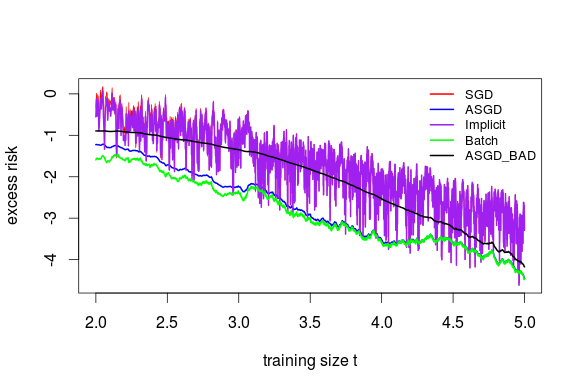
\includegraphics[scale=0.55]{./img/2a_updates.png}
\captionof{figure}{Excess risk for different update methods. SGD and Implicit methods exposes a very unstable behaviors. General relative behaviors of methods are nonetheless reproduced compared to Xu. Excess risk and trainining size t on $log_{10}$ scale.}
\endgroup


\subsection{SGD methods on regression}

\begingroup
\centering
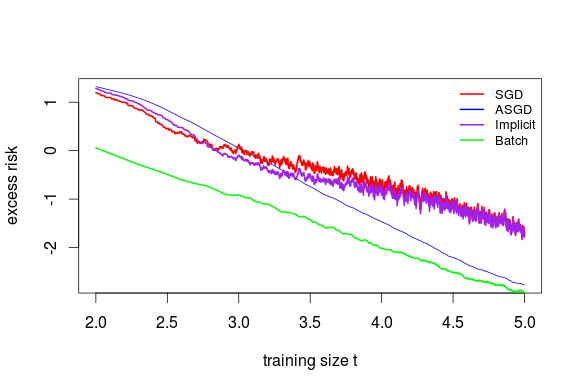
\includegraphics[scale=0.55]{./img/2b_sgd_updates.png}
\captionof{figure}{Excess risk for different update methods. Like in Xu, SGD starts with better performance than ASGD but eventually performs worse for high training size (Implicit does slightly better than SGD). Batch is doing better overall. Excess risk and trainining size t on $log_{10}$ scale.}
\endgroup

\begingroup
\centering
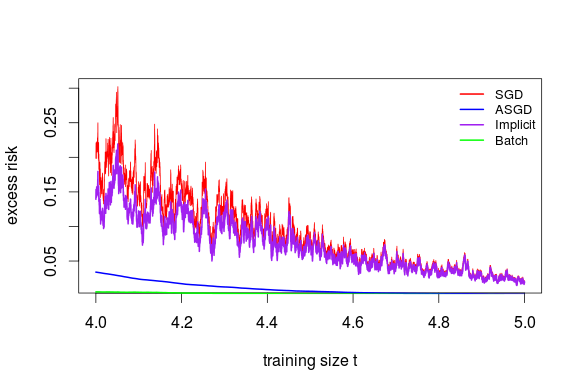
\includegraphics[scale=0.55]{./img/2b_sgd_upd_10e4.png}
\captionof{figure}{Excess risk zoom on training size superior to $10^4$.}
\endgroup



%----------------------------------------------------------------------------------------

%\end{multicols}

\end{document}
